\chapter{Depth-first search}
\label{chap:depthfirst}

De eerste methode die onderzocht is voor het zoeken naar een augmented path is de Depth-first search methode. Deze methode zal, zoals de naam suggereert, de diepte in gaan op zoek naar $t$. Dit is ge\"illustreerd in figuur \ref{fig:depthFirstTree}, de getallen op de knopen geven aan in welke volgorde ze doorzocht zijn.

\begin{figure}[h]
 \centering
 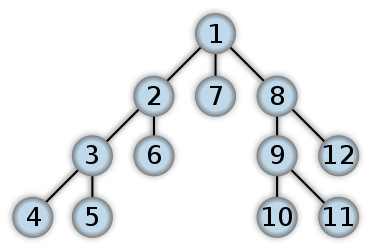
\includegraphics[width=0.5\linewidth]{depthfirst/depthfirsttree}
 \caption{Depth-first doorzoeken van een boom}
 \label{fig:depthFirstTree}
\end{figure}

De recursieve methode DFS verwacht als invoer een graaf $g$, een startknoop $s$, een eindknoop $t$ en een map $parents$. Deze map wordt later gebruikt om de weg van $t$ naar $s$ te vinden. Bij elke aanroep zal $s$ gelabeld worden als \textit{EXPLORED} $\land$. Hierna zullen alle aanliggende kanten van $s$ bijlangs gegaan worden om te kijken of hier nog een eventueel pad mogelijk is. Dit wordt gedaan door te kijken naar de overstaande knoop $w$ via $e$. Wanneer $w$ gelabeld is als \textit{UNEXPLORED} en de kant $e$ nog een capaciteit heeft, is hier een pad mogelijk. $e$ zal nu gezet worden als de parent van $w$ en daarnaast ook nog gelabeld worden als \textit{DISCOVERY} $\land$. Nu zal een recursieve aanroep gedaan worden met de parameters respectievelijk $g$, $w$, $t$ en $parents$.
Als $w$ niet gelabeld is als \textit{UNEXPLORED} zal $e$ gelabeld worden als \textit{BACK} $\land$.

\section{Pseudocode}
De pseudocode waar de code op gebaseerd is, is te vinden in algoritme \ref{alg:DFS}.
Wanneer het eindpunt $t$ bereikt is kan het algoritme stoppen. Nu kan met behulp van de $parents$ gezocht worden naar een pad van $s$ naar $t$ door te kijken wat de parent edge $e$ is van $t$. Nu zal gekeken worden naar de parent edge van de overstaande van $t$ via edge $e$. Door dit te doen tot er geen parent edge is zal $s$ bereikt worden.

\begin{algorithm}[h]
\caption{Depth-first search Algorithm}
\label{alg:DFS}
\begin{algorithmic}
\REQUIRE Input: Graph g, Start vertex s, End vertex t, HashMap parents with vertexes and its parent edges

\STATE Label s as \textit{EXPLORED}
\FORALL{edge $e \in s.incidentEdges$}
\IF{e is not labeled as \textit{UNEXPLORED} $\land$ s.residualCapacity(e) $> 0$}
\STATE w $\gets$ g.opposite(s, e)
\IF{w is labeled as \textit{UNEXPLORED}}
\STATE label $e$ as \textit{DISCOVERY} edge
\STATE set $e$ as parent of $w$ in the hashmap parents
\STATE recursive call with g, w, t and parents
\ELSE
\STATE label $e$ as \textit{BACK} edge
\ENDIF
\ENDIF
\ENDFOR
\end{algorithmic}
\end{algorithm}

\subsection{Analyse}

Figuur \ref{fig:DFS_graph1} en \ref{fig:DFS_graph2} laten de uitkomst zien van de analyse.

\begin{figure}[h]
	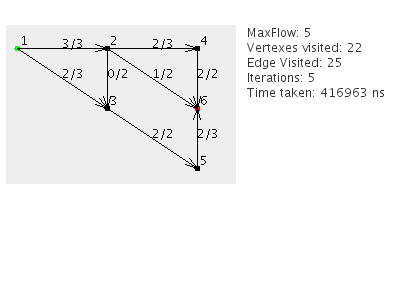
\includegraphics[width=0.5\linewidth]{depthfirst/DFS_graph1}
	\centering
	\caption{Analyse van de eerste graaf}
	\label{fig:DFS_graph1}
\end{figure}

\begin{figure}[h]
	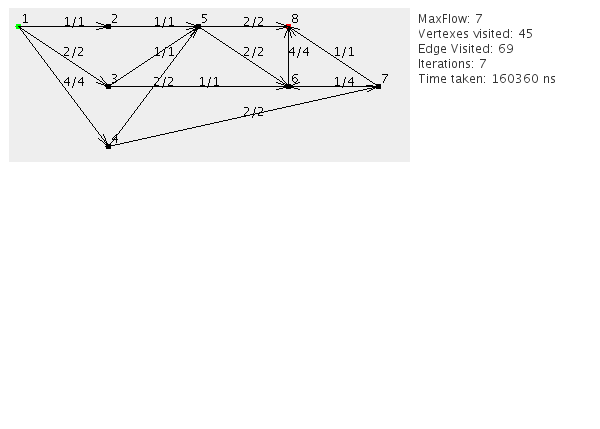
\includegraphics[width=0.5\linewidth]{depthfirst/DFS_graph2}
	\centering
	\caption{Analyse van de tweede graaf}
	\label{fig:DFS_graph2}
\end{figure}

